\documentclass[12pt]{article}
\usepackage[utf8]{inputenc}
\usepackage{float}
\usepackage{amsmath}
\usepackage{graphicx}

\usepackage[hmargin=3cm,vmargin=6.0cm]{geometry}
\topmargin=-2cm
\addtolength{\textheight}{6.5cm}
\addtolength{\textwidth}{2.0cm}
\setlength{\oddsidemargin}{0.0cm}
\setlength{\evensidemargin}{0.0cm}
\usepackage{indentfirst}
\usepackage{amsfonts}

\begin{document}

\section*{Student Information}

Name : Emre Geçit

ID : 2521581

\section*{Question 1}
Design a Turing machine which recognizes the language $L = \{0^N1^N | N \geq 1\}$.

$\Sigma = \{0, 1, \sqcup\}$, means that you cannot write any other symbol than these symbols.
\subsection*{States:}
\begin{itemize}
    \item State 0 (Initial state): If the tape head is on a 0, changes it with a blank space, moves the tape head to right, and passes to the state 1. If it is on a blank space, passes to the acceptance state.
    \item State 1: This state's task is finding the right end of the string. After finding the rightmost symbol in the string, the machine passes to state 2.
    \item State 2: If the tape head is on a 1, changes it with a blank space, moves the tape head to left, and passes to the state 3. If it is on a blank space, passes to the acceptance state.
    \item State 3: This state's task is finding the left end of the string. After finding the leftmost symbol in the string, the machine passes to state 0.
\end{itemize}
Note that in these descriptions, undefined transititons leads to rejection of the string.
\begin{figure}[H]
    \caption{Turing machine which recognizes the language $L = \{0^N1^N | N \geq 1\}$}
    \centering
    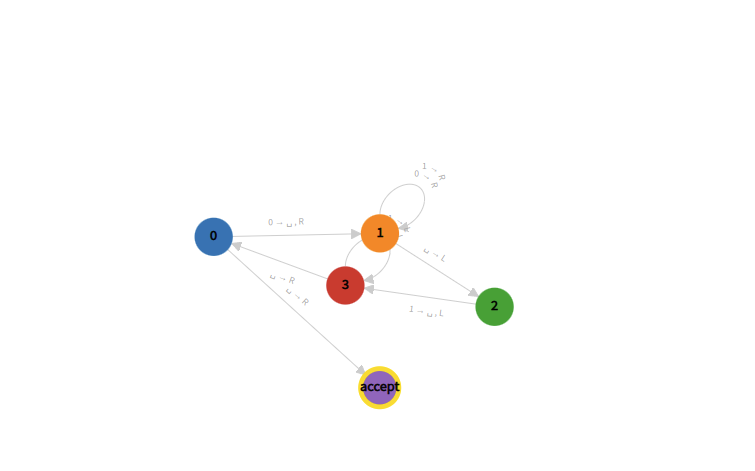
\includegraphics[width=12cm]{Q1/turingmachine.io_.png}    
\end{figure}
\newpage
\subsection*{Sample inputs:}
\begin{figure}[H]
    \caption{Input = 000111}
    \centering
    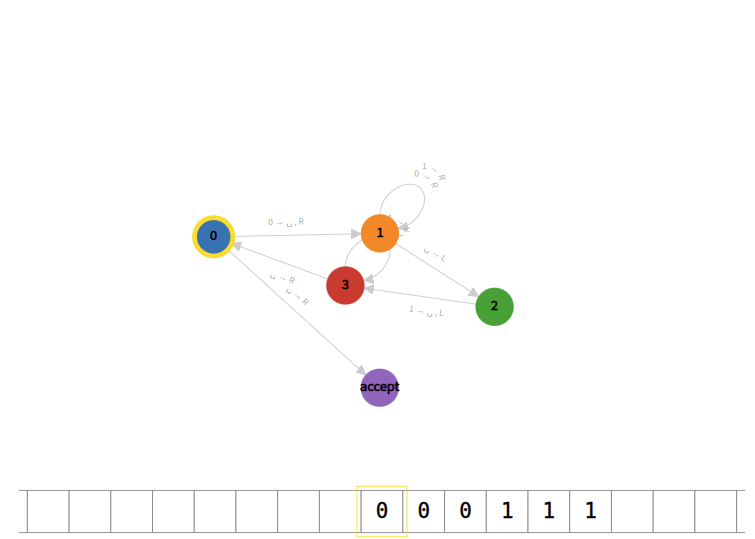
\includegraphics[width=12cm]{Q1/000111.png}    
\end{figure}
\begin{figure}[H]
    \caption{000111 accepted}
    \centering
    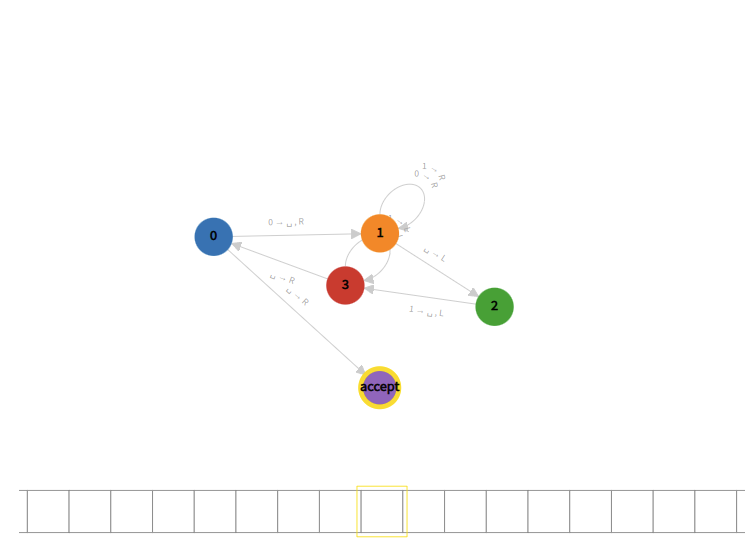
\includegraphics[width=12cm]{Q1/000111o.png}    
\end{figure}
\begin{figure}[H]
    \caption{Input = 0000111}
    \centering
    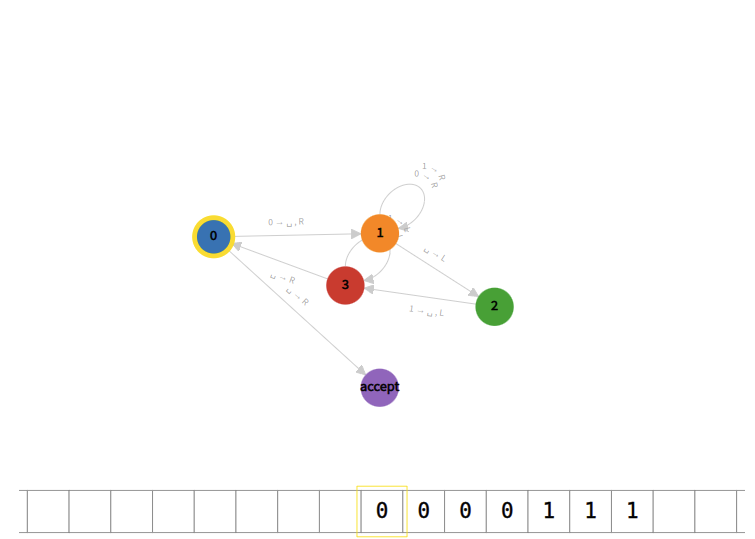
\includegraphics[width=12cm]{Q1/0000111.png}    
\end{figure}
\begin{figure}[H]
    \caption{0000111 rejected}
    \centering
    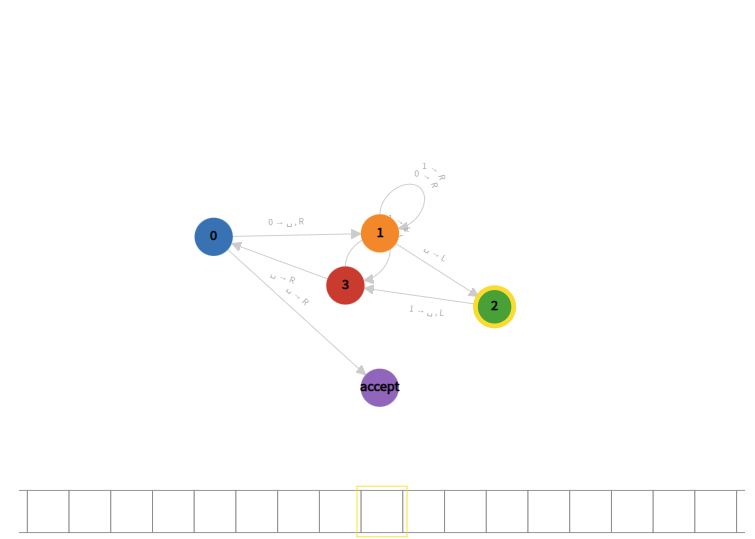
\includegraphics[width=12cm]{Q1/0000111o.png}    
\end{figure}
\begin{figure}[H]
    \caption{Input = 000011111}
    \centering
    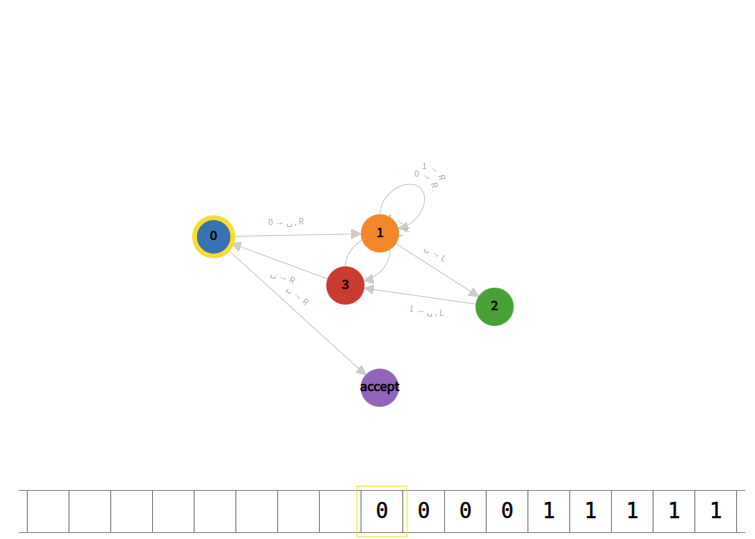
\includegraphics[width=12cm]{Q1/000011111.png}  
\end{figure}
\begin{figure}[H]
    \caption{000011111 rejected}
    \centering
    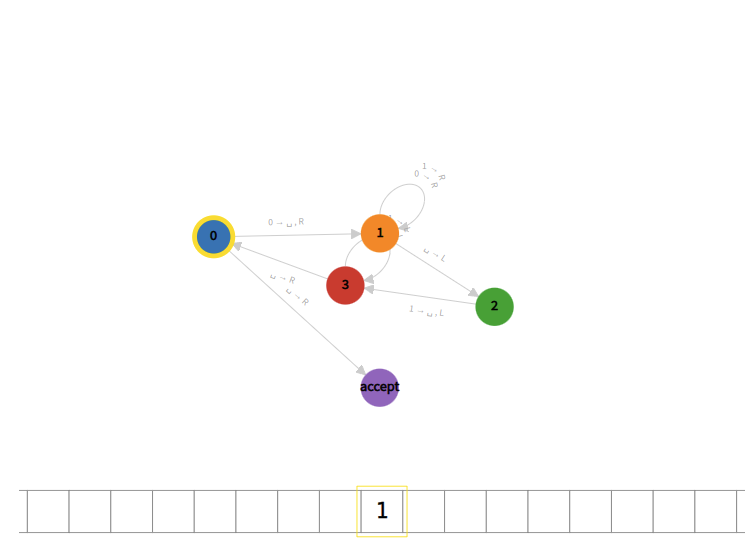
\includegraphics[width=12cm]{Q1/000011111o.png}  
\end{figure}
\begin{figure}[H]
    \caption{Input = 0001110}
    \centering
    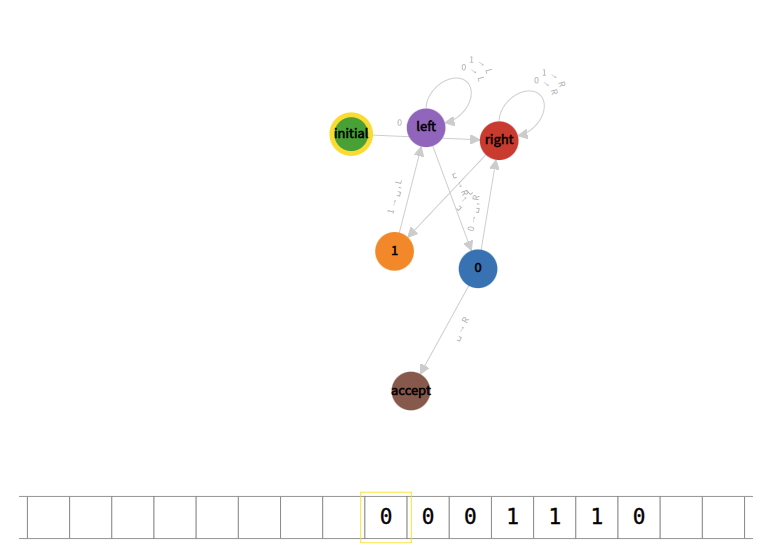
\includegraphics[width=12cm]{Q1/0001110.png}  
\end{figure}
\begin{figure}[H]
    \caption{0001110 rejected}
    \centering
    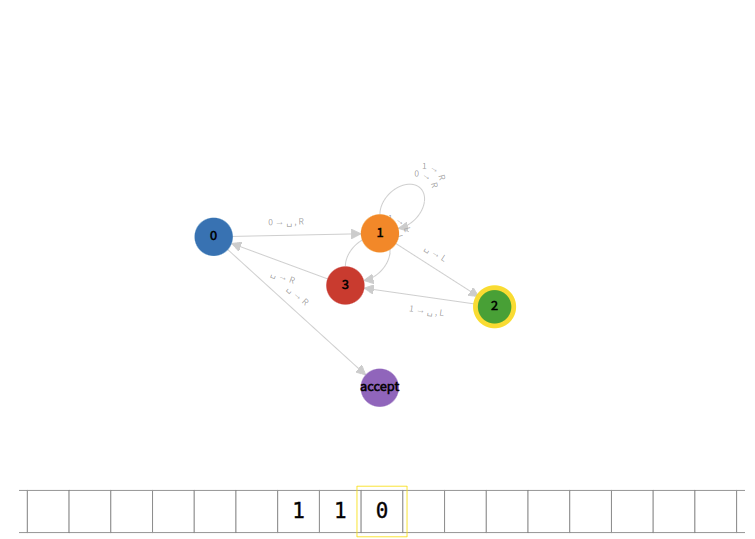
\includegraphics[width=12cm]{Q1/001101o.png}  
\end{figure}
\begin{figure}[H]
    \caption{Input = 100011}
    \centering
    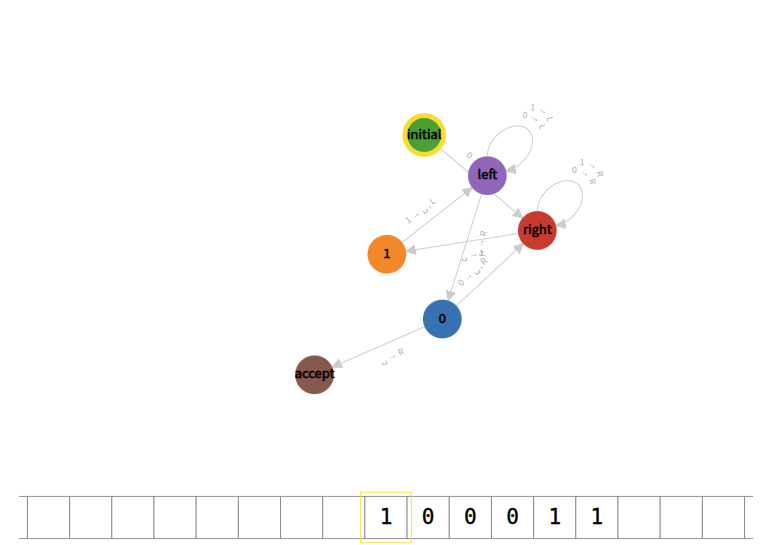
\includegraphics[width=12cm]{Q1/100011.png}
\end{figure}
\begin{figure}[H]
    \caption{100011 rejected}
    \centering
    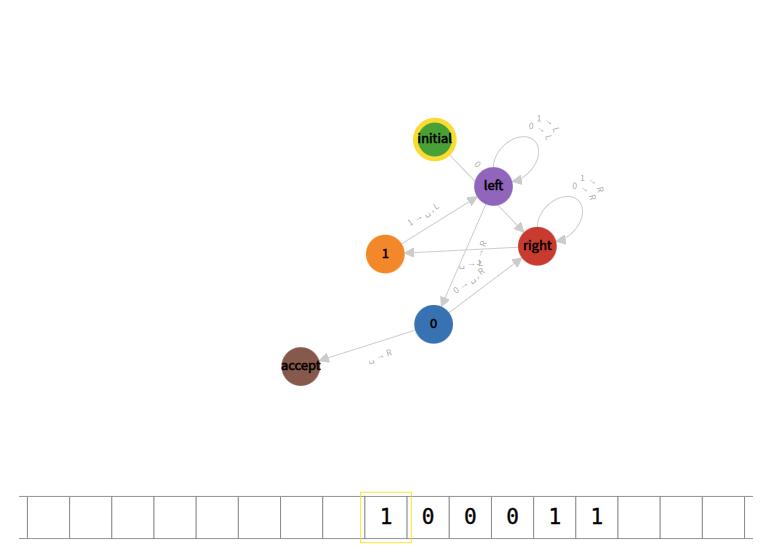
\includegraphics[width=12cm]{Q1/100011o.png}
\end{figure}
\section*{Question 2}
Design a Turing machine that computes the function $f(w) = ww^R$, $\Sigma(w) = \{0, 1\}$.
\subsection*{States:}
\begin{itemize}
    \item convert{\_}symbols (Initial state): This states changes all zeros with x's, and all ones with y's. Then, it moves the tape head to the right.
    \item find{\_}last{\_}character: This state finds the last symbol that has not been copied and passes to copy{\_}y if the tape head is on a y, or to copy{\_}x if the tape head is on a x.
    \item copy{\_}y: This state goes to the end of the tape, and writes a 1.
    \item copy{\_}x: This state goes to the end of the tape, and writes a 0.
\end{itemize}
\begin{figure}[H]
    \caption{Turing machine which computes the function $f(w) = ww^R$}
    \centering
    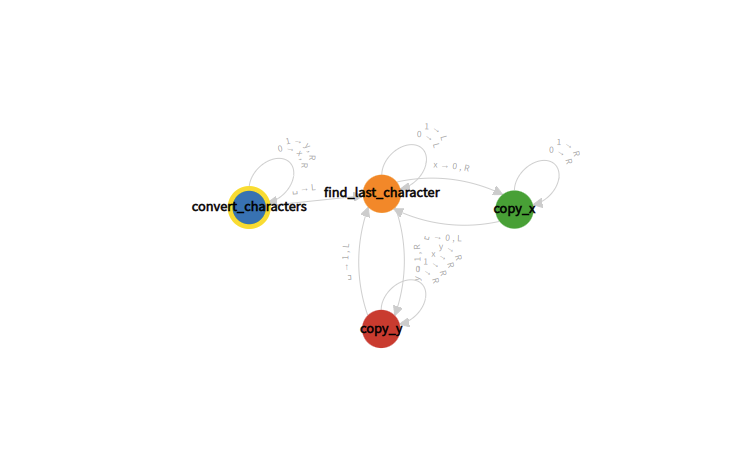
\includegraphics[width=17cm]{Q2/turingmachine.io_.png}
\end{figure}
\newpage
\subsection*{Sample inputs:}
\begin{figure}[H]
    \caption{Input = 1011}
    \centering
    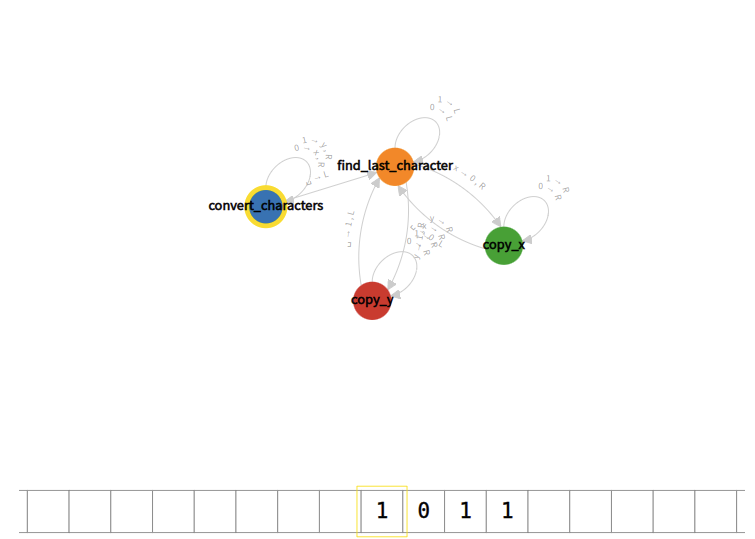
\includegraphics[width=12cm]{Q2/1011.png}
\end{figure}
\begin{figure}[H]
    \caption{Output = 10111101}
    \centering
    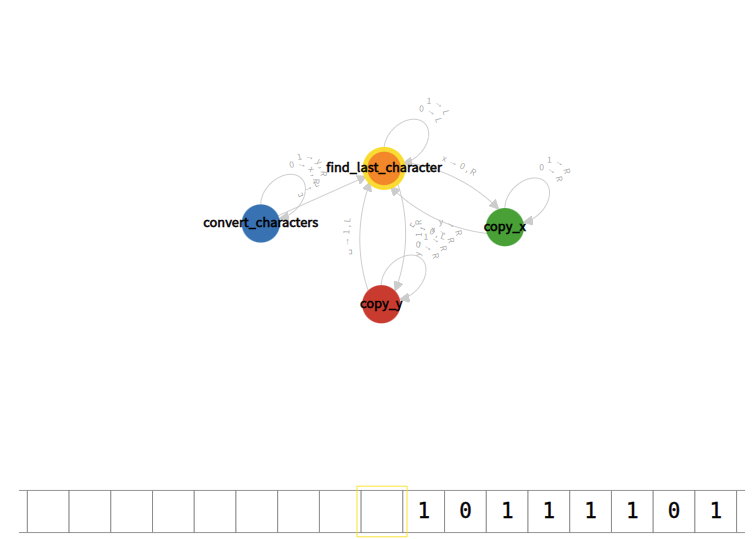
\includegraphics[width=12cm]{Q2/10111101.png}
\end{figure}
\begin{figure}[H]
    \caption{Input = 1110}
    \centering
    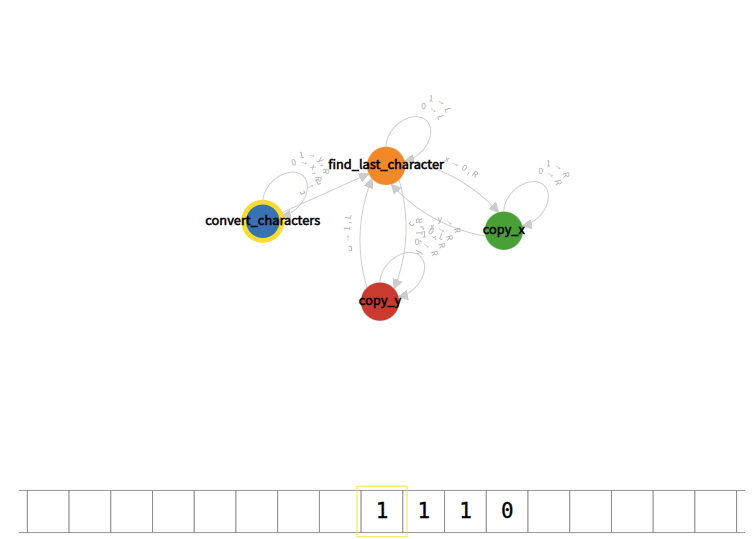
\includegraphics[width=12cm]{Q2/1110.png}
\end{figure}
\begin{figure}[H]
    \caption{Output = 11100111}
    \centering
    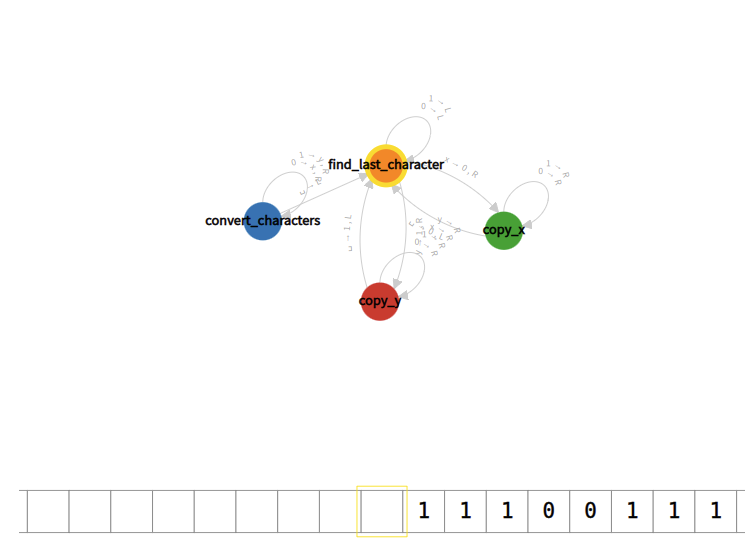
\includegraphics[width=12cm]{Q2/11100111.png}
\end{figure}
\begin{figure}[H]
    \caption{Input = 0101}
    \centering
    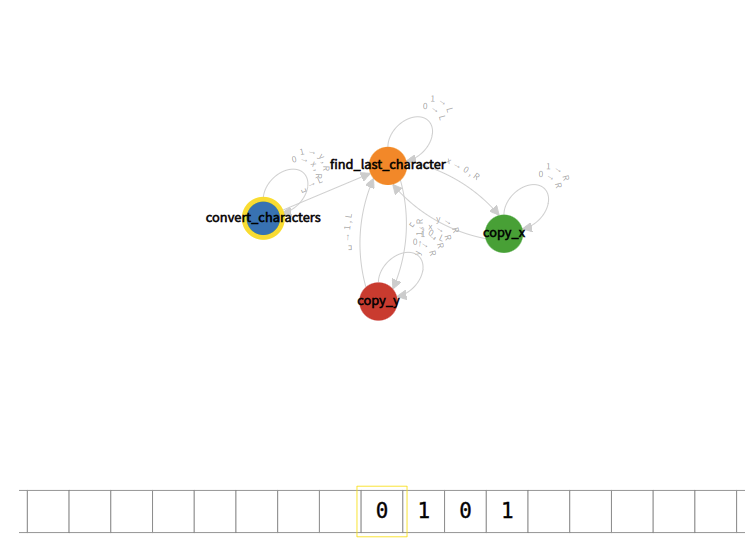
\includegraphics[width=12cm]{Q2/0101.png}
\end{figure}
\begin{figure}[H]
    \caption{Output = 01011010}
    \centering
    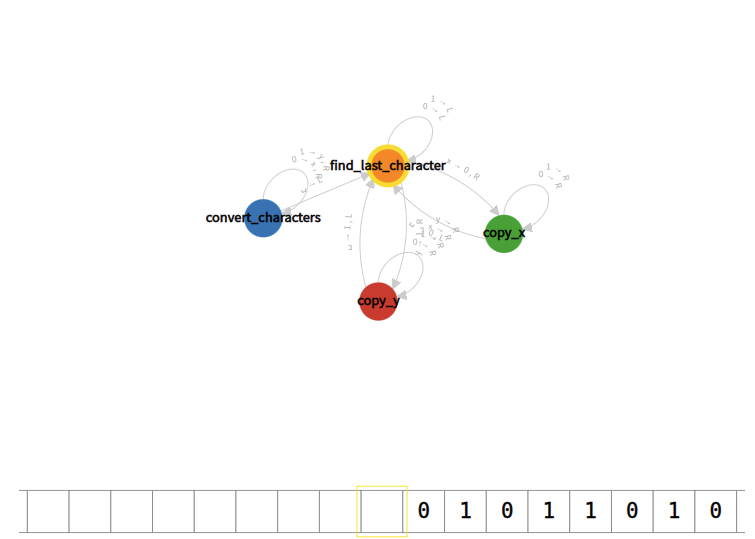
\includegraphics[width=12cm]{Q2/01011010.png}
\end{figure}
\begin{figure}[H]
    \caption{Input = 1010}
    \centering
    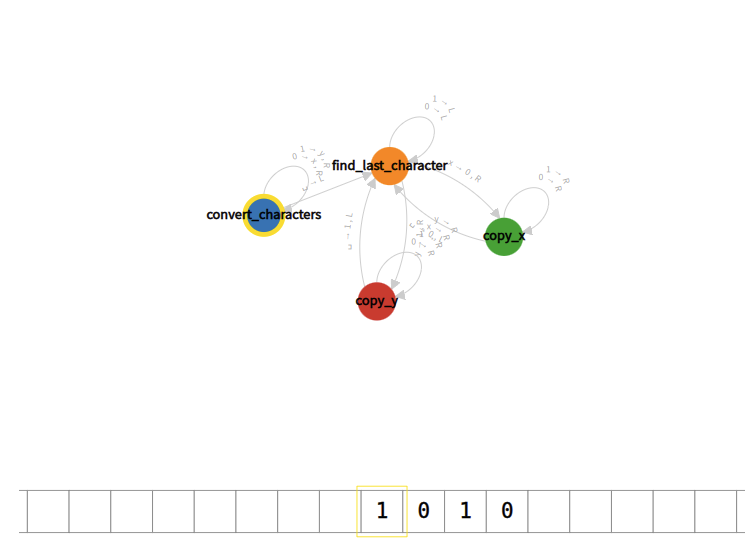
\includegraphics[width=12cm]{Q2/1010.png}
\end{figure}
\begin{figure}[H]
    \caption{Output = 10100101}
    \centering
    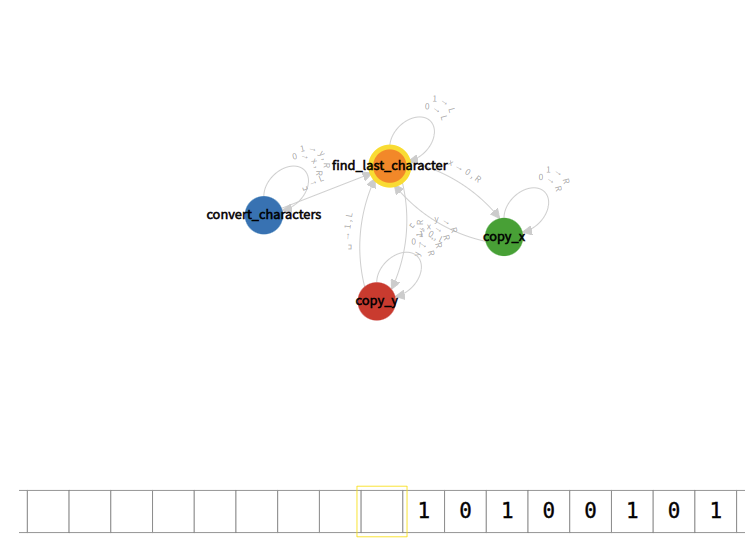
\includegraphics[width=12cm]{Q2/10100101.png}
\end{figure}
\begin{figure}[H]
    \caption{Input = 1010001}
    \centering
    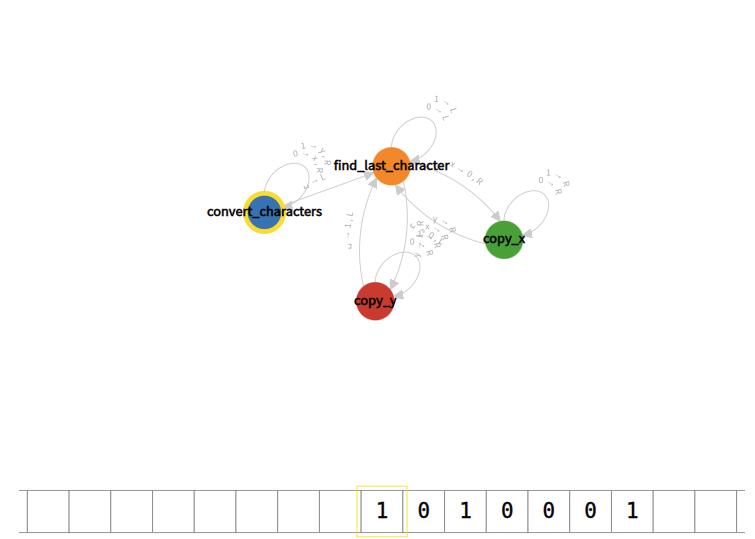
\includegraphics[width=12cm]{Q2/1010001.png}
\end{figure}
\begin{figure}[H]
    \caption{Output = 10100011000101}
    \centering
    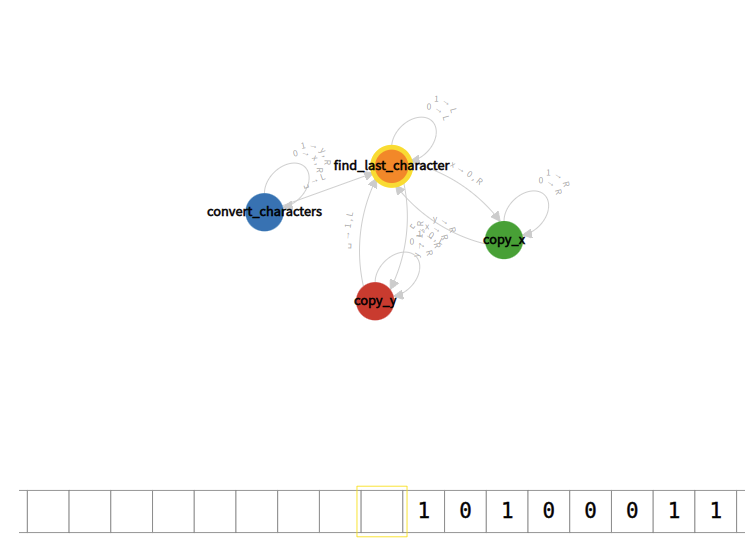
\includegraphics[width=12cm]{Q2/10100011000101.png}
\end{figure}
\begin{figure}
    \caption{Input = 00111}
    \centering
    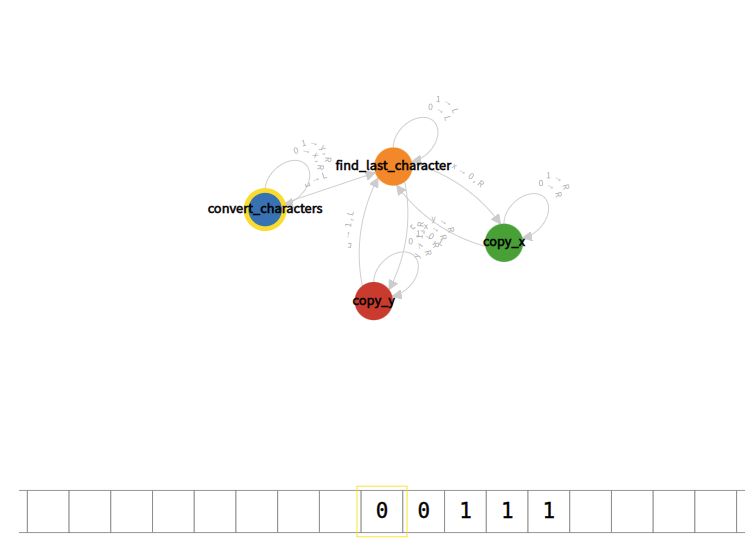
\includegraphics[width=12cm]{Q2/00111.png}
\end{figure}
\begin{figure}
    \caption{Output = 0011111100}
    \centering
    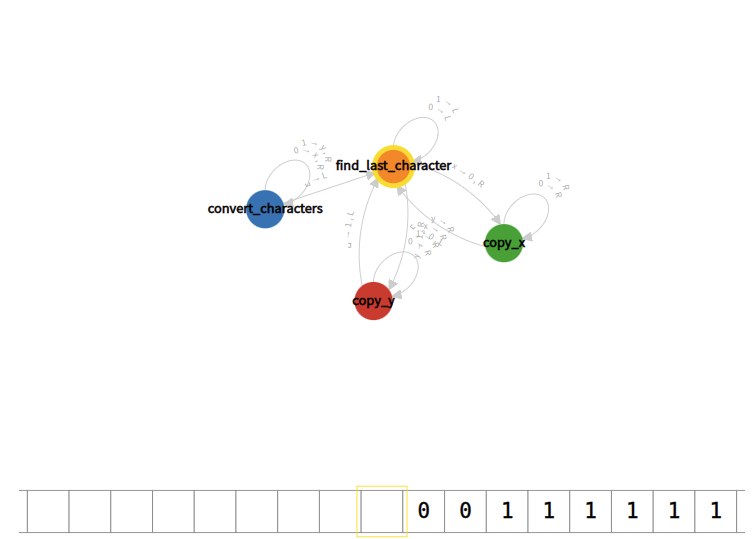
\includegraphics[width=12cm]{Q2/0011111100.png}
\end{figure}
\newpage
\section*{Question 3}
Formally define a Turing machine with a 2-dimensional tape, its configurations, and its computation.
Define what it means for such a machine to decide a language L. Show that t steps of this machine,
starting on an input of length n, can be simulated by a standard Turing machine in time that is
polynomial in t and n.
\subsection*{Solution:}
\paragraph{1)} A Turing machine with a 2-dimensional tape is a quintuple $(K, \Sigma, \delta, s, H)$, where

\begin{itemize}
    \item $K$ is a finite set of states;
    \item $\Sigma$ is a finite set of symbols containing the blank symbol $\sqcup$ but not containing $\uparrow$, $\nearrow$, $\rightarrow$, $\searrow$, $\downarrow$, $\swarrow$, $\leftarrow$, or $\nwarrow$;
    \item $s\in K$ is the initial state;
    \item $H \subseteq K$ is the set of halting states;
    \item $\delta$, the transititon function, $\delta: (K - H) \times  \Sigma \to (K - H) \times (\Sigma \cup \{\uparrow, \nearrow, \rightarrow, \searrow, \downarrow, \swarrow, \leftarrow, \nwarrow\})$;
\end{itemize}

\paragraph{2)} A Turing machine with a 2-dimensional M is said to decide a language $L$ if $L = L(M)$ and M halts on every input.????????????

\paragraph{3)} First of all, we should define the mechanics of the classical Turing machine $M'$, that will simulate our 2-dimensional machine $M$.

The tape of $M'$ must somehow contain all information in all tapes of $M$. A simple way of achieving this is by thinking that the $M'$ is divided into several tracks, with each "track" devoted to the simulation of a row of the 2d-tape.

After defining formal specifications of $M'$, we should fill in the input tape of $M'$ before starting the simulation.
\end{document}